\documentclass[a4paper,10pt]{article}

%% Paquetes Adicionales %%

\usepackage[spanish]{babel}
\selectlanguage{spanish}
\spanishdecimal{.}
\addto\captionsspanish{\def\tablename{Cuadro}}
\usepackage{fancyhdr}
\usepackage{graphics}
\usepackage[dvips]{graphicx}
\usepackage[normal]{caption2}
\usepackage{amsfonts,amssymb,amsmath,amsthm}
\usepackage[T1]{fontenc}
\usepackage{moreverb}

%% Declaracion de comandos %%

\newtheorem{lema}{Lema}
\newtheorem{teor}{Teorema}
\newtheorem{propos}{Proposici\'on}
\newtheorem{corol}{Corolario}

\newcommand{\mivec}[1]{\mathbf{#1}}
\newcommand{\vers}[1]{\mivec{\check{#1}}}
\newcommand{\deriv}[2]{\frac{\mathrm{d}#1}{\mathrm{d}#2}}
\newcommand{\expo}[1]{~10^{#1}}
\newcommand{\uni}[1]{\mathrm{#1}} 

\newcommand{\prop}[1]{\begin{propos} #1 \end{propos}}
\newcommand{\teo}[1]{\begin{teor} #1 \end{teor}}
\newcommand{\cor}[1]{\begin{corol} #1 \end{corol}}
\newcommand{\lem}[1]{\begin{lema} #1 \end{lema}}

%% Encabezado y Pie de Pagina %%

\pagestyle{plain}
\lhead{}
\chead{}
\rhead{}
\cfoot{\thepage}
\renewcommand{\footrulewidth}{0.4pt}

%%\author{Juan Ignacio Go\~ni}

\makeindex

%% Titulo %%
\begin{document}
\title{{\ Taller de proyecto final \\ Robot recolector de residuos \\ Placa controladora de motor DC}}

%\date{}

%% Comienzo del documento %%

\maketitle

\begin{abstract}
En el presente se establecen las especificaciones para la placa controladora de motor DC.
Se expone el circuito de la placa, explica funcionamiento y se muestran posibles usos.

\textbf{Palabras Clave: }\emph{Robot, residuos, motor de continua, driver, controladora, encoder, protocolo, serial, rs-232, daisy chain}.
\end{abstract}

% \thispagestyle{fancy}

%% COMIENZO DEL TEXTO %%

% Intro
\section{Introducci\'on}
\label{introduccion}

Un robot recolector de basura tiene una necesidad principal que es poder movilizarse por el terreno y debido a que el desplazamiento se realiza
mediante ruedas, el control de los motores que las impulsan es una necesidad b\'asica.

En las siguientes secciones se explica y detalla cada uno de los aspectos tenidos en cuenta para dise\~nar y crear la placa controladora de motores
de corriente continua para el robot.

% La placa base -> generica
\section{La placa gen\'erica}
\label{placagenerica}

Como se explica en el documento \emph{Placa m\'odulo gen\'erico}, la comunicaci\'on es un aspecto importante y se uso dicha placa como base y modelo
para el dise\~no de la controladora de motores de continua. El circuito como se puede apreciar en las secciones \ref{esquematico} y \ref{circuito},
comparten gran parte de la disposici\'on l\'ogica y funcional de los componentes. Esta cuestion ayuda en gran medida tanto al armado y manipulaci\'on
de las placas al mantener la compatibilidad modular entre las mismas.

Se utiliza el mismo microcontrolador que la placa gen\'erica y se comparten los switches de configuraci\'on para los modos de comunicaci\'on y programaci\'on.

% Lo que se necesita - control de velocidad, encoders, historicos, sentido de giro, consumo
\section{Requerimientos funcionales}
\label{requerimientos}

Como requerimientos m\'inimos se encontraba el poder controlar la velocidad de forma estable de los motores bajo demanda, determinar el sentido de giro
de los motores, poder obtener informaci\'on sobre el consumo y tener acceso a un historico de vueltas o cuentas de encoder que tuvo el motor.

Tambi\'en era deseable poder delegar cierta l\'ogica en el control, determinando la cantidad de movimiento que se deseaba que el motor realizara y
asegurarse una mejor resolucion para el control de posici\'on.

% Comandos especificos del protocolo
\section{Comandos del protocolo para la controladora}
\label{comandos}

Como se explica en el documento \emph{Protocolo de comunicaci\'on}, cada placa tiene sus comandos propios para el intercambio de comandos y envio de
informaci\'on.
Entre otros se encuentran los comandos necesarios para especificar y obtener la velocidad y sentido de giro, seteo y lectura del historico de cuentas
del encoder, cuentas para detener el motor y control sobre la alarma de consumo de corriente del motor.

% El motor
\section{El motor de corriente continua}
\label{motor}

El motor elegido es un motor de corriente continua

***VER QUE MOTOR VA A IR*** - consumo y demas...

% La caja reductora
\section{La caja reductora}
\label{caja}

La caja de reducci\'on es permite convertir las altas revoluciones del motor en una menor cantidad pero a un mayor torque.
Esto es necesario porque la mayor potencia del motor se obtiene al girar a altas revoluciones, pero dicha velocidad no es de utilidad
para impulsar las ruedas debido al peque\~no torque y alta velocidad.

***VER QUE CAJA TIENE EL MOTOR QUE VA A IR*** - relacion, torque y demas...

% Encoders para el control de velocidad
\section{Encoders en el motor}
\label{encoders}

Los encoders son de gran utilidad para poder medir el \'angulo de giro que realiz\'o el motor en cierto intervalo de tiempo.
Esto se traduce en que si se conoce la relaci\'on entre una vuelta de motor y una vuelta de rueda y sus dimensiones,
se puede controlar la velocidad del robot. La precisi\'on con la que se mide la velocidad depende en gran medida de la resoluci\'on
del encoder y del control de tiempo en el microcontrolador.

***VER QUE ENCODERS TIENE EL MOTOR QUE VA A IR*** - cuentas por vuelta, tipo de sensado

% Driver y los diodos
\section{Driver de potencia}
\label{driver}

Debido a que el consumo del motor excede la potencia que puede erogar el microcontrolador, se necesita un driver de potencia que soporte dicho consumo.
El driver elegido es el \emph{L298N} con las salidas puenteadas en configuraci\'on paralela para aumentar la potencia a $4A$. Los diodos \emph{FR304}
fueron los elegidos como rectificadores complemento al driver.

El consumo de corriente es medido mediante el conversor anal\'ogico digital incluido en el microcontrolador.

Se dej\'o la posibilidad de realizar una modificaci\'on al circuito, agregando un divisor de voltaje para dar una referencia al \emph{ADC} y poder ajustar
el rango de lectora del mismo al requerido por el circuito.

% Circuito, esquematico, alimentacion y conectores
\section{Alimentaci\'on}
\label{alimentacion}

La alimentaci\'on principal de la l\'ogica de la placa es 7 a 20 voltios, con la posibilidad de alimentarla directamente 
con 5 voltios por uno de los pines del conector.
La alimentaci\'on del motor es por un conector distinto aislando as\'i el ruido generado por los motores de la l\'ogica.

En la figura \ref{borneras} se muestran las borneras y en los cuadros \ref{alimentacionLogica} y \ref{alimentacionMotor} el pinout de las mismas.

\begin{figure}
\centering
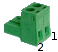
\includegraphics[scale=1]{bornera2.png}
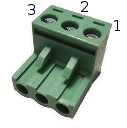
\includegraphics[scale=.5]{bornera3.png}
\caption{Borneras de 2 y 3 pines para la alimentaci\'on de la placa}
\label{borneras}
\end{figure}

\begin{table}
\begin{center}
\begin{tabular}{|c|c|}
\hline
Pin & Voltaje \\
\hline
1 & GND \\
\hline
2 & 12v (depende del motor) \\
\hline
\end{tabular}
\caption{Alimentaci\'on del motor}
\label{alimentacionMotor}
\end{center}
\end{table}

\begin{table}
\begin{center}
\begin{tabular}{|c|c|}
\hline
Pin & Voltaje \\
\hline
1 & GND \\
\hline
2 & 5v \\
\hline
3 & 7v a 12v \\
\hline
\end{tabular}
\caption{Alimentaci\'on de la l\'ogica}
\label{alimentacionLogica}
\end{center}
\end{table}

La regulaci\'on interna de voltaje para la l\'ogica realiza por medio de un regulador 7805 de igual forma que se hace en la placa gen\'erica.

\section{Configuraci\'on}
\label{configuracion}

El header de programaci\'on \emph{P1} se utiliza para conectar la placa con el programador y debuguer de c\'odigo \emph{ICD2} como se explica en la secci\'on \ref{programador}.

Los headers \emph{P2} y \emph{P3} vinculan las resistencias \emph{R5} y \emph{R6} del divisor de voltaje con le voltaje de referencia para el 
conversor anal\'ogico digital del microcontrolador.

El header de pines \emph{P4} se utiliza para la conexi\'on con el motor, explicado en el cuadro \ref{pinoutMotor}.

\begin{table}
\begin{center}
\begin{tabular}{|c|c|c|c|}
\hline
Pin & Se\~nal & Pin & Se\~nal \\
\hline
1 & Motor\_B & 2 & Motor\_A \\
\hline
3 & Motor\_IDX & 4 & No conectado \\
\hline
5 & Encoder\_B & 6 & GND \\
\hline
7 & Encoder\_A & 8 & GND \\
\hline
9 & +5 VCC & 10 & GND \\
\hline
\end{tabular}
\caption{Pinout del header del motor}
\label{pinoutMotor}
\end{center}
\end{table}

El switch \emph{S3} se utiliza para determinar el papel de la placa dentro de la cadena (modo \emph{LINK} o modo \emph{LAST}).
El switch \emph{S2} se utiliza para asociar los pines del microcontrolador con el canal de datos del header de programaci\'on (modo \emph{ICD2}) o con el encoder
elegido en el \emph{S4} (Encoder\_A o Encoder\_B).

\section{Esquem\'atico}
\label{esquematico}

En la figura \ref{schema1} se detalla el esquem\'atico del microcontrolador y el conexionado el header de programaci\'on.

En la figura \ref{schema2} se muestra el m\'odulo de comunicaci\'on y el conexionado con los conectores para conformar la cadena \emph{Daisy chain}.

La figura \ref{schema3} muestra el esquem\'atico del driver y el header del motor.

En la figura \ref{schema4} se ve el header del divisor de voltaje para el voltaje de referencia del ADC del microcontrolador.

En la figura \ref{schema5} se muestra la fuente de alimentaci\'on y borneras.

\begin{figure}
\centering
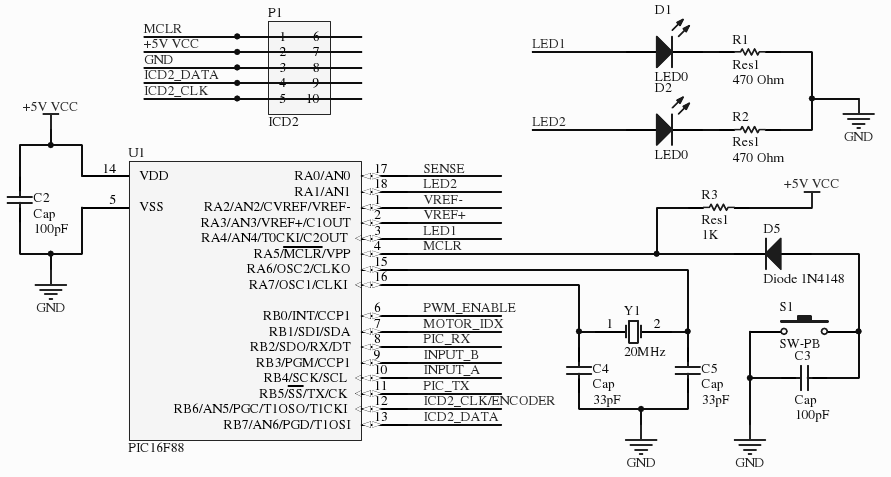
\includegraphics[scale=.3]{schemaMicro.png}
\caption{Microcontrolador y header de programaci\'on}
\label{schema1}
\end{figure}

\begin{figure}
\centering
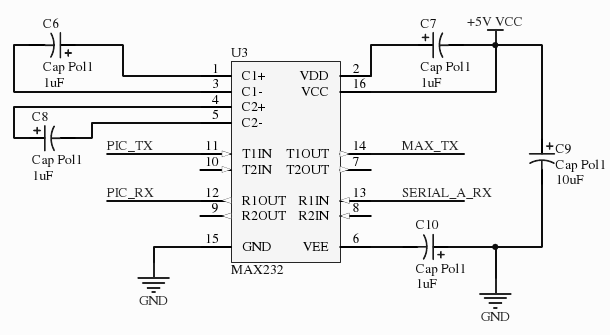
\includegraphics[scale=.28]{schemaComm1.png}
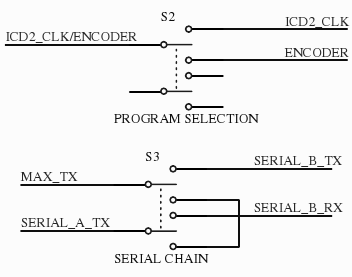
\includegraphics[scale=.28]{schemaComm2.png}
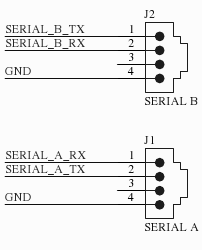
\includegraphics[scale=.28]{schemaComm3.png}
\caption{Comunicaci\'on, switch de modo y conectores de entrada y salida}
\label{schema2}
\end{figure}

\begin{figure}
\centering
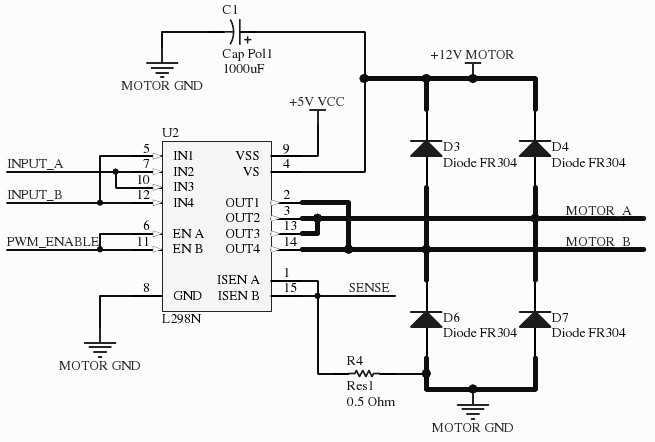
\includegraphics[scale=.3]{schemaDriver.png}
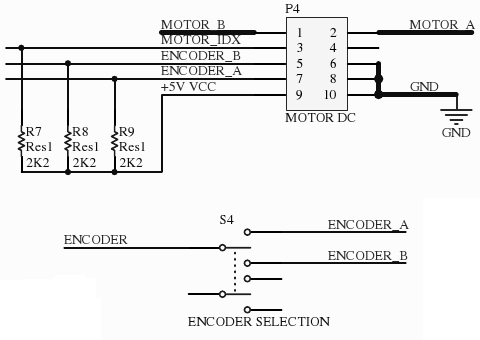
\includegraphics[scale=.3]{schemaMotorEncoder.png}
\caption{Driver y header de conexi\'on con el motor}
\label{schema3}
\end{figure}

\begin{figure}
\centering
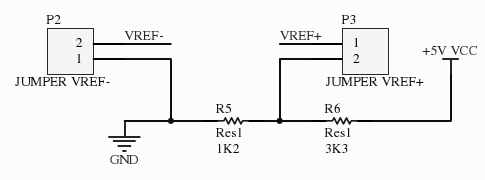
\includegraphics[scale=.3]{schemaADC.png}
\caption{Header que conecta el divisor de voltaje con el microcontrolador para definir el voltaje de referencia}
\label{schema4}
\end{figure}

\begin{figure}
\centering
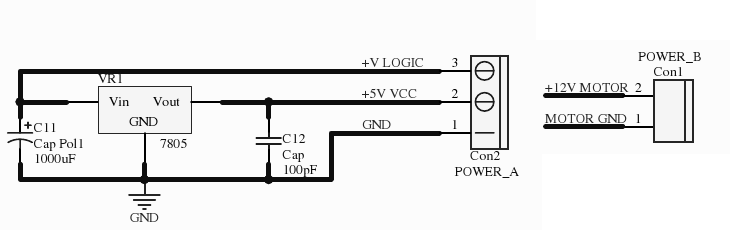
\includegraphics[scale=.3]{schemaFuente.png}
\caption{Fuente de alimentaci\'on de la l\'ogica y motor}
\label{schema5}
\end{figure}

\section{Circuito}
\label{circuito}

En la figura \ref{componentes} se muestra la m\'ascara de componentes de la placa.
En la figura \ref{capas} se muestran ambas capas de la placa.

\begin{figure}
\centering
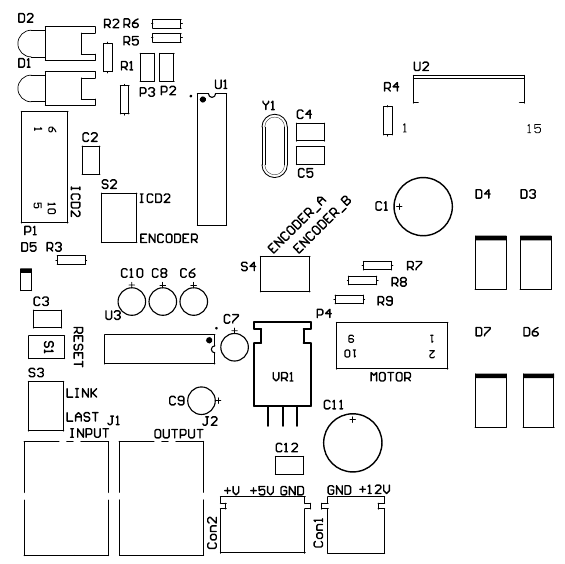
\includegraphics[scale=.3]{componentes.png}
\caption{M\'ascara de componentes}
\label{componentes}
\end{figure}

\begin{figure}
\centering
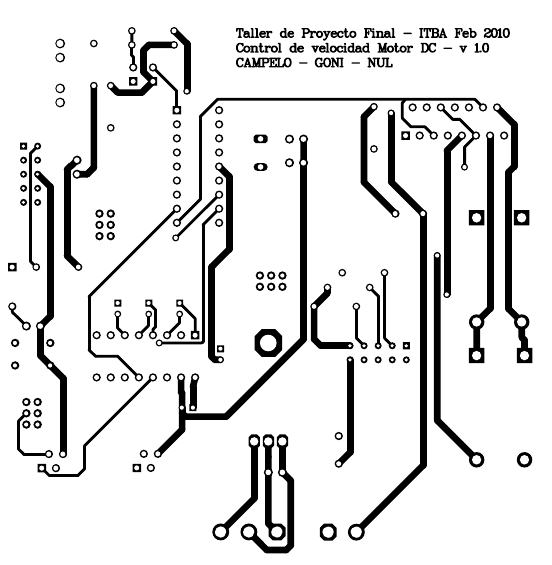
\includegraphics[scale=.3]{top.png}
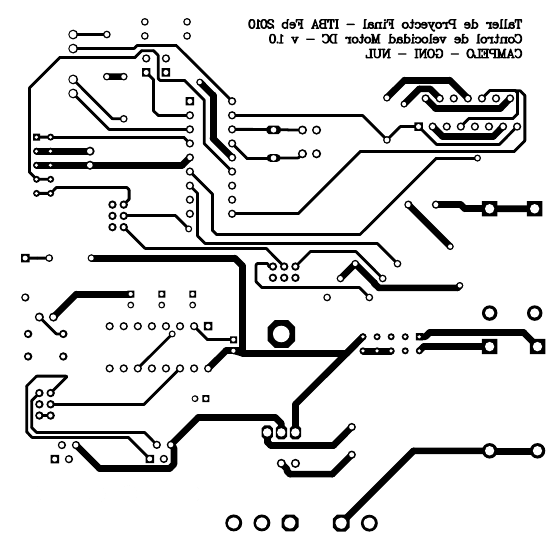
\includegraphics[scale=.3]{bottom.png}
\caption{Capas superior e inferior de la placa}
\label{capas}
\end{figure}

\section{C\'odigo b\'asico}
\label{codigo}

Debido a que la placa fue pensada como punto de partida, se provee del c\'odigo utilizado como base para la programaci\'on de las otras placas controladoras.

{\scriptsize
\begin{verbatimtab}
//CCS PCM V4.023 COMPILER

#define CARD_GROUP	MOTOR_DC	// Ver protocol.h
#define CARD_ID		0		// Valor entre 0 y E

// Descripcion de la placa
#define DESC		"CONTROL MOTOR DC 1.0" // Maximo DATA_SIZE bytes

/* Modulo Motor - main.c
 * PIC16F88 - MAX232 - L298 - MR-2-60-FA
 *
 *                               PIC16F88
 *                .------------------------------------.
 *          VREF -|RA2/AN2/CVREF/VREF           RA1/AN1|- MOTOR:CHA_B
 *           LED -|RA3/AN3/VREF+/C1OUT          RA0/AN0|- L298:SEN
 *           LED -|RA4/AN4/T0CKI/C2OUT    RA7/OSC1/CLKI|- XT CLOCK pin1, 27pF to GND
 * RST/ICD2:MCLR -|RA5/MCLR/VPP           RA6/OSC2/CLKO|- XT CLOCK pin2, 27pF to GND
 *           GND -|VSS                              VDD|- +5v
 *   L298:ENABLE -|RB0/INT/CCP1       RB7/AN6/PGD/T1OSI|- ICD2:PGD
 *     MOTOR:IDX -|RB1/SDI/SDA  RB6/AN5/PGC/T1OSO/T1CKI|- ICD2:PGC/MOTOR:CHA_A
 *  MAX232:R1OUT -|RB2/SDO/RX/DT           RB5/SS/TX/CK|- MAX232:T1IN
 * L298:INPUT_B/ -|RB3/PGM/CCP1             RB4/SCK/SCL|- L298:INPUT_A
 *     ICD2:PGM   '------------------------------------'
 *    
 */

#include <16F88.h>
#DEVICE ADC = 10
#include <stdio.h>
#include <string.h>
#include <stdlib.h>

#fuses HS,NOWDT,NOPROTECT,NOLVP
#use delay (clock=20000000)

#use rs232(BAUD=115200,PARITY=N,XMIT=PIN_B5,RCV=PIN_B2,BITS=8,ERRORS,TIMEOUT=1,STOP=1,UART1)
#use fast_io(A)
#use fast_io(B)

#byte porta=0x05
#byte portb=0x06

// MAX232
#bit tx=portb.5
#bit rx=portb.2

// Led
#bit led1=porta.3
#bit led2=porta.4

// L298
#bit inputA=portb.4
#bit inputB=portb.3
#bit enable=portb.0
#bit sensor=porta.0

// Motor inuts
#bit motorIDX=portb.1
#bit channelA=portb.6
#bit channelB=porta.1

#include <../../protocolo/src/protocol.c>
/*
** Variables definidas en protocol.c

short reset; // Variable para hacer el reset
short crcOK; // Informa si el CRC del paquete parseado fue correcto
short sendResponse; // Informa que no debe mandarse la respuesta automatica

char buffer[MAX_BUFFER_SIZE];	// Buffer de recepcion de comandos
int buffer_write;				// Indice de escritura
int buffer_read;				// Indice de lectura
int data_length;				// Largo de los datos en el buffer

struct command_t command; 	// Comando parseado
struct command_t response; 	// Respuesta

** Implementar las siguientes funciones (usadas por el protocolo)

void init(); // Inicializa puertos y variables
void doCommand(struct command_t * cmd); // Examina y ejecula el comando

***/

#define MAX_CONSUMPTION	150
#define MAX_CONSUMPTION_COUNT	5

// Correcion de la cantidad de cuentas por segundo en base al periodo del TMR0
#define INTERVAL_CORRECTION	5

// Girar -> clockwise or unclockwise
// Intercambiar entre el motor derecho y el izquierdo
#define CLOCKWISE	1
#define UNCLOCKWISE	-1

// Sentido de giro del motor
signed int turn;
// Cantidad de overflows del TMR0
long tmr0_ticks;
// Valor acumulado del ADC - Consumo aprox
long adc_value;
// Ultimo valor del consumo
long last_consumption;
// Valor de duty del PWM
signed long duty;
// Cantidad de cuentas del encoder medidas por intervalo
signed long counts_real;
// Cantidad de cuentas del encoder esperadas por intervalo
signed long counts_expected;
// Cantidad de cuentas del encoder historicas (32 bits)
signed int32 counts_total;
// Cantidad de cuentas del encoder restantes para deterner el motor
signed long counts_to_stop;
// Cantidad de cuentas del encoder desde el ultimo intevalo
signed long last_counts;
signed long last_counts2;
// Tengo una cantidad de cuentas para hacer?
short counts_check;
// Corrijo el PWM segun lo esperado?
short correct_duty;
// Indica que hay que enviar una alarma de consumo
short consumption_alarm;
// Cuenta cuantas alarmas se enviaron
int alarm_count;
// Indica que hay que avisar que el motor se detuvo
short shutdown_alarm;
// Indica si se apagaron los motores por el alto consumo
short motor_shutdown;

// Variables temporales
signed int32 * tmp32;
signed long * tmp16;

/* Setea el PWM */
void SetPWM(signed long pwm);

// Interrupcion del Timer0
#INT_RTCC
void Timer0_INT()
{
	// Seteo el valor para que interrumpa cada 6.25ms
	set_timer0(12);
	
	// Comienza la lectura del ADC
	read_adc(ADC_START_ONLY);
	
	// Agrego al historico de cuentas el ultimo acumulado
	counts_real = get_timer1();
	counts_total += (counts_real - last_counts2) * turn;
	last_counts2 = counts_real;
	
	// Tengo una cantidad de cuentas para hacer?
	if (counts_check == 1)
	{
		// Verifico si pasaron las cuentas que se habian pedido
		if (counts_to_stop < 1)
		{
			// Detengo el motor
			counts_check = 0;
			counts_to_stop = 0;
			counts_expected = 0;
			duty = 0;
			SetPWM(duty);
			correct_duty = 0;
			last_counts = 0;
		} else {
			counts_real = get_timer1();
			counts_to_stop -= (counts_real - last_counts);// * turn;
			correct_duty = 1;
			last_counts = counts_real;
		}
	} else {
		correct_duty = 1;
	}
	
	// Tomo la muestra
	adc_value += read_adc(ADC_READ_ONLY);
	
	if (++tmr0_ticks == 32)
	{
		// Entra cada 200ms

		// Obtengo la cantidad de cuentas desde la ultima entrada
		counts_real = get_timer1();
		set_timer1(0);
		last_counts = 0;
		last_counts2 = 0;
		// Promedio el consumo segun la cantidad de tmr0_ticks
		last_consumption = adc_value / tmr0_ticks;
		
		if (last_consumption >= MAX_CONSUMPTION)
		{
			consumption_alarm = 1;
			if (alarm_count++ == MAX_CONSUMPTION_COUNT)
			{
				motor_shutdown = 1;
				alarm_count = 0;
				consumption_alarm = 0;
				shutdown_alarm = 1;
			}	
		}
		
		tmr0_ticks = 0;

		// Mantengo el consumo promedio desde que arranque y borro el temporal
		adc_value = 0;

		// Corrijo el PWM segun lo esperado
		if ((correct_duty == 1) && (counts_real != counts_expected))
		{
			duty += (counts_expected - counts_real) * 5;
			if (duty > 1023L)
				duty = 1023;
			else if (duty < 0)
				duty = 0;
			SetPWM(duty * turn);
		} else if ((counts_expected == 0) && (duty != 0)) {		
			SetPWM(duty = 0);
		}	
	}
	return;
}

void init()
{
	// Inicializa puertos
	set_tris_a(0b11100111);
	set_tris_b(0b11100110);

	// ***ADC***
	setup_port_a(sAN0);//|VSS_VREF);
	setup_adc(ADC_CLOCK_INTERNAL);
	set_adc_channel(0);
	setup_adc_ports(sAN0);
	// Deberia usar VREF_A2... probar
	setup_vref(VREF_HIGH | 8); // VREF a 2.5V -> no hay cambios...
	
	// ***PWM***
	setup_ccp1(CCP_PWM);
	// Seteo al PWM con f: 4.88 kHz, duty = 0
	set_pwm1_duty(0);
	setup_timer_2(T2_DIV_BY_4, 255, 1);

	// ***TIMER1 - ENCODER COUNTER***
	// Seteo el Timer1 como fuente externa y sin divisor
	setup_timer_1(T1_EXTERNAL | T1_DIV_BY_1);
	set_timer1(0);

	// ***TIMER0 - TIME BASE***
	// Seteo el Timer0 como clock -> dt = 6.25ms
	setup_counters(RTCC_INTERNAL, RTCC_DIV_128);
	set_timer0(12);
	// Interrupcion sobre el Timer0
	enable_interrupts(INT_RTCC);

	// Habilito las interrupciones
	enable_interrupts(GLOBAL);
	
	// Variable para hacer el reset
	reset = false;

	// Sentido de giro del motor
	turn = CLOCKWISE;
	// Cantidad de overflows del TMR0
	tmr0_ticks = 0;
	// Valor acumulado del ADC - Consumo aprox
	adc_value = 0;
	last_consumption = 0;
	// Valor de duty del PWM
	duty = 0;
	// Cantidad de cuentas del encoder esperadas por intervalo
	counts_expected = 0;
	// Cantidad de cuentas del encoder totales
	counts_total = 0;
	// Cantidad de cuentas del encoder restantes para deterner el motor
	counts_to_stop = 0;
	// Cantidad de cuentas del encoder desde el ultimo intevalo
	last_counts = 0;
	last_counts2 = 0;
	// Tengo una cantidad de cuentas para hacer?
	counts_check = 0;
	// Corrijo el PWM segun lo esperado?
	correct_duty = 1;
	// Indica que hay que enviar una alarma de consumo
	consumption_alarm = 0;
	// Cuenta cuantas alarmas se enviaron
	alarm_count = 0;
	// Indica que hay que enviar una alarma de consumo
	shutdown_alarm = 0;
	// Indica si se apagaron los motores por el alto consumo
	motor_shutdown = 0;

	return;	
}	

/* Setea el duty del PWM segun el valor. Positivo o negativo determina el sentido */
void setPWM(signed long pwm)
{
	if (pwm < 0)
	{
		inputA = 0;
		inputB = 1;
	} else {
		inputA = 1;
		inputB = 0;
	}
	
	if (motor_shutdown == 1)
	{
		pwm = 0;
	} else {
		pwm = (abs(pwm));
		
		if (pwm > 1023L)
			pwm = 1023;
	}

	set_pwm1_duty(pwm);
	
	return;
}

void main()
{
	// Placa Generica - Implementacion del protocolo
	init();

	// Init del protocol
	initProtocol();

counts_expected = 30;

	// FOREVER
	while(true)
	{
		// Hace sus funciones -> interrupcion
	
		// Enviar alarma de alto consumo
		if (consumption_alarm == 1)
		{
			/* Indica al controlador principal que hay un consumo extremo en el motor,
			posiblemente un atasco del motor o de la rueda.
			:DATO:
			Numero entero positivo de 16 bits en el rango desde 0x0000 hasta
			0x03FF, que representa el consumo ante el que sono la alarma.
			:RESP:
			-
			*/
			command.len = MIN_LENGTH + 2;
			command.to = MAIN_CONTROLLER;
			command.from = THIS_CARD;
			command.cmd = DC_MOTOR_MOTOR_STRESS_ALARM;
			// A la posicion 0 dentro de command.data la tomo como signed long *
			tmp16 = (command.data);
			// Le asigno el valor del ultimo consumo del motor
			(*tmp16) = last_consumption;
			command.crc = generate_8bit_crc((char *)(&command), command.len, CRC_PATTERN);
			consumption_alarm = 0;
			// Envio del comando
			send(&command);
		}
		
		// Enviar aviso de motor apagado
		if (shutdown_alarm == 1)
		{
			/* Indica al controlador principal que el motor ha sido apagado debido al alto
			consumo. Enviado luego de sucesivos avisos del comando DC_MOTOR_MOTOR_STRESS_ALARM.
			:DATO:
			Numero entero positivo de 16 bits en el rango desde 0x0000 hasta
			0x03FF, que representa el consumo ante el que sono la alarma.
			:RESP:
			-
			*/
			command.len = MIN_LENGTH + 2;
			command.to = MAIN_CONTROLLER;
			command.from = THIS_CARD;
			command.cmd = DC_MOTOR_MOTOR_SHUT_DOWN_ALARM;
			// A la posicion 0 dentro de response->data la tomo como signed long *
			tmp16 = (command.data);
			// Le asigno el valor del ultimo consumo del motor
			(*tmp16) = last_consumption;
			command.crc = generate_8bit_crc((char *)(&command), command.len, CRC_PATTERN);
			shutdown_alarm = 0;
			// Envio del comando
			send(&command);
		}
			
		// Protocolo
		runProtocol(&command);
	}

	return;
}

/* Verifica que el comando sea valido y lo ejecuta */
void doCommand(struct command_t * cmd)
{
	int crc, i, len;
		
	// Calculo del CRC
	crc = generate_8bit_crc((char *)cmd, cmd->len, CRC_PATTERN);
	
	// CRC ok?
	if (cmd->crc != crc)
	{		
		// Creo respuesta de error
		response.len = MIN_LENGTH + cmd->len + 2 + 1;
		response.to = cmd->from;
		response.from = THIS_CARD;
		response.cmd = COMMON_ERROR;
		response.data[0] = 0x00;
		// Agrego el paquete que contiene el error de CRC
		response.data[1] = cmd->len;
		response.data[2] = cmd->to;
		response.data[3] = cmd->from;
		response.data[4] = cmd->cmd;
		// Campo data
		len = cmd->len - MIN_LENGTH;
		for (i = 0; i < len; i++)
			response.data[5 + i] = (cmd->data)[i];
		// CRC erroneo
		response.data[5 + len] = cmd->crc;
		// CRC esperado
		response.data[5 + len + 1] = crc;
		// CRC de la respuesta
		response.crc = generate_8bit_crc((char *)(&response), response.len, CRC_PATTERN);
	
		crcOK = false;
		return;
	}

	crcOK = true;
	
	// Minimo todos setean esto
	response.len = MIN_LENGTH;
	response.to = cmd->from & 0x77;
	response.from = THIS_CARD;
	response.cmd = cmd->cmd | 0x80;

	switch (cmd->cmd)
	{
		// Comandos comunes
		case COMMON_INIT: 
			init();
			// Enviar la descripcion de la placa en texto plano
			strcpy(response.data, DESC);
			response.len += strlen(response.data);
		break;
		case COMMON_RESET: 
			// Enviar la descripcion de la placa en texto plano
			strcpy(response.data, DESC);
			response.len += strlen(response.data);
			// Reset!
			reset = true;
		break;
		case COMMON_PING: 
			// No hace falta hacer mas nada
		break;
 		case COMMON_ERROR:
			// Por ahora se ignora el comando
		break;
		
		/* Comandos especificos */

 		case DC_MOTOR_SET_DIRECTION:
			/* Seteo del sentido de giro del motor
			:DATO:
			0x00 para sentido horario o 0x01 para sentido anti-horario.
			:RESP:
			-
			*/
			if (((cmd->data)[0] & 0x01) == 0)
			{
				turn = CLOCKWISE;
			} else {
				turn = UNCLOCKWISE;
			}
		break;
 		case DC_MOTOR_SET_DC_SPEED:
			/* Seteo de la velocidad del motor en cuentas del encoder por segundo
			:DATO:
			0x00 para sentido horario o 0x01 para sentido anti-horario. Numero 
			entero de 16 bits con signo, que representa la velocidad en cuentas 
			por segundos.
			:RESP:
			-
			*/
			if (((cmd->data)[0] & 0x01) == 0)
			{
				turn = CLOCKWISE;
			} else {
				turn = UNCLOCKWISE;
			}
			// A la posicion 1 dentro de cmd->data la tomo como signed long *
			tmp16 = (cmd->data) + 1;
			// Le asigno el valor de la velocidad ajustada a 1 segundo
			counts_expected = (*tmp16) / INTERVAL_CORRECTION;
			// Habilita el motor
			motor_shutdown = 0;
		break;
 		case DC_MOTOR_SET_ENCODER:
			/* Seteo de la cantidad de cuentas historicas del encoder
			:DATO:
			Numero entero de 32 bits con signo, con el valor para setear en el
			historico del encoder.
			:RESP:
			-
			*/
			// A la posicion 0 dentro de cmd->data la tomo como signed int32 *
			tmp32 = (cmd->data);
			// Le asigno el valor de las cuentas historicas
			counts_total = (*tmp32);
		break;
 		case DC_MOTOR_GET_ENCODER:
			/* Obtener la cantidad de cuentas historicas del encoder
			:DATO:
			-
			:RESP:
			Numero entero de 32 bits con signo, que representa el valor historico
			del encoder.
			*/
			// A la posicion 0 dentro de response->data la tomo como signed int32 *
			tmp32 = (response.data);
			// Le asigno el valor de las cuentas historicas
			(*tmp32) = counts_total;
			// Corrijo el largo del paquete
			response.len += 4;
		break;
 		case DC_MOTOR_RESET_ENCODER:
			/* Resetear las cuentas historicas a cero
			:DATO:
			-
			:RESP:
			-
			*/
			counts_total = 0;
		break;
 		case DC_MOTOR_SET_ENCODER_TO_STOP:
			/* Seteo de cuantas cuentas debe girar hasta detenerse
			:DATO:
			Numero entero de 16 bits con signo, que representa la cantidad de
			cuentas del encoder restantes para que el motor se detenga.
			:RESP:
			-
			*/
			// A la posicion 0 dentro de cmd->data la tomo como signed long *
			tmp16 = (cmd->data);
			// Le asigno el valor de la velocidad ajustada a 1 segundo
			counts_to_stop = (*tmp16);
			// Habilito el chequeo de cuentas para detener el motor
			counts_check = 1;
		break;
 		case DC_MOTOR_GET_ENCODER_TO_STOP:
			/* Obtener la cantidad de las cuentas restantes que quedan por 
			realizar hasta detenerse.
			:DATO:
			-
			:RESP:
			Numero entero de 16 bits con signo, que representa la cantidad
			de cuentas del encoder restantes para detener el motor.
			*/
			// A la posicion 0 dentro de response->data la tomo como signed long *
			tmp16 = (response.data);
			// Le asigno el valor de la velocidad ajustada a 1 segundo
			(*tmp16) = counts_to_stop;
			// Corrijo el largo del paquete
			response.len += 2;
		break;
 		case DC_MOTOR_DONT_STOP:
			/* Deshace los comandos DC_MOTOR_DONT_STOP y DC_MOTOR_GET_ENCODER_TO_STOP, 
			deshabilita el conteo de cuentas para frenar y sigue en el estado actual.
			:DATO:
			-
			:RESP:
			-
			*/
			counts_check = 0;
		break;
 		case DC_MOTOR_MOTOR_CONSUMPTION:
			/* Numero entero positivo de 16 bits en el rango desde 0x0000 hasta
			0x03FF, que representa el consumo promedio del ultimo segundo.
			:DATO:
			-
			:RESP:
			-
			*/
			// A la posicion 0 dentro de response->data la tomo como signed long *
			tmp16 = (response.data);
			// Le asigno el valor del ultimo consumo del motor
			(*tmp16) = last_consumption;
			// Corrijo el largo del paquete
			response.len += 2;
		break;
 		/*case DC_MOTOR_MOTOR_STRESS_ALARM:
		break;
 		case DC_MOTOR_MOTOR_SHUT_DOWN_ALARM:
		break;*/
 		case DC_MOTOR_GET_DC_SPEED:
			/* Obtiene la velocidad del motor en cuentas del encoder por segundo
			:DATO:
			0x00 para sentido horario o 0x01 para sentido anti-horario. Numero
			entero de 16 bits con signo, que representa la velocidad en cuentas
			por segundos.
			:RESP:
			-
			*/
			// Sentido de giro del motor
			if (turn == CLOCKWISE)
			{
				(response.data)[0] = 0x00;
			} else {
				(response.data)[0] = 0x01;
			}
			// A la posicion 1 dentro de response->data la tomo como signed long *
			tmp16 = (response.data) + 1;
			// Le asigno el valor de la velocidad ajustada a 1 segundo
			(*tmp16) = counts_real * INTERVAL_CORRECTION;
			// Corrijo el largo del paquete
			response.len += 2;
		break;

		default:
			response.len++;
			response.cmd = COMMON_ERROR;
			response.data[0] = 0x01; // Comando desconocido
		break;
	}	

	// CRC de la respuesta
	response.crc = generate_8bit_crc((char *)(&response), response.len, CRC_PATTERN);

	return;
}
\end{verbatimtab}
}

El c\'odigo incluye al archivo \emph{protocolo.c} que se puede encontrar en la documentaci\'on de la placa gen\'erica.

\end{document}